\section{DCT anvendelse} \label{sec:DCTAnvendelse}
I dette afsnit undersøges den praktiske anvendelse af DCT, jævnfør kapitel \ref{chapter:DCT}, hvilket udføres på billedet af Lena, se figur \vref{fig:lena-grid-8x8}. Billedet har dimensionerne $ 512 \times \SI{512}{pixel}$, hvilket indledningsvist opdeles i $8 \times 8$ undermatricer. Endvidere er der $ 64 \cdot 64$ matricer af $8 \times 8$, hvilket giver $64 \cdot 64 \cdot 8 \cdot 8 = 262.144$ pixels totalt.

De følgende regneoperationer bliver kun udført på den røde farvekanal og første $8 \times 8$ undermatrix for at vise princippet ved brugen af metoden. Ved gentagelse med resten af undermatricerne og de resterende to farvekanaler opnås en komprimering af det fulde farvebillede. Repetitionerne af beregningerne udelades, da dette blot er et eksempel. Derimod \textit{vises} resultatet af komprimeringen for hele billedet, efter regneeksemplet med undermatricen er udført. For at skabe overblik over komprimeringen ses komprimeringsalgoritmen herunder:
\begin{table}[!h]
\centering
\begin{tabular}{lll}
\hline
\multicolumn{3}{l}{\textbf{Algoritme: Komprimering vha. DCT}}                           \\ \hline
\\
\multicolumn{1}{|l}{1.}        & Input:                     & Billede, $A$: $m \times n$ pixels             \\
\multicolumn{1}{|l}{2.}        & Output:                    & Komprimeret fil       \\
                               &                            &                        \\
\multicolumn{2}{|l}{\textit{Komprimering}}                  &                        \\
\multicolumn{1}{|l}{3.}        & Opdeling:                  & Billede opdeles i farvekanaler og $8 \times 8$ matricer \\
\multicolumn{1}{|l}{4.}        & Centrering omkring 0:      & $A = A - 128$ indgangsvist    \\
\multicolumn{1}{|l}{5.}        & DCT:              & $B = U \boldsymbol{\cdot} A \boldsymbol{\cdot} U^T$  \\
\multicolumn{1}{|l}{6.}        & Kvantisering:              & $\lfloor C_{(i,\ j)} \rceil = \frac{B_{(i,\ j)}}{Q_{(i,\ j)}}$ afrundet\\
\multicolumn{1}{|l}{7.}        & Entropi kodning:           & $C$ komprimeres vha. Huffman til en fil              \\
\multicolumn{1}{|l}{8.}        & Gentagelse:                & Ovenstående gentages for samtlige $8 \times 8$ matricer\\
\end{tabular}
\label{tb:Algoritme-Komprimering-DCT}
\end{table}

Den specifikke undermatrix i følgende eksempel ligger i øverste venstre hjørne, jævnfør figur \vref{fig:lena-grid-8x8}. Første værdi for hver indgang, dvs. den røde kanal, findes vha. vores Python-program og følgende undermatrix, $A_{1,1}$, fremkommer.

\begin{figure}[!h]
\begin{minipage}[b]{0.27\linewidth}
\centering

\includegraphics[width=\textwidth]{Billeder/LenaAnvendelse/RED8x8/lena1-R8x8-org.png}
\caption{Oprindelig - Visuel.}
\label{fig:lena1-R8x8-org-visuel}
\end{minipage}
\hspace{0.5cm}
\begin{minipage}[b]{0.45\linewidth}
\centering
\[A_{1,1}=\begin{bmatrix}
226 & 226 & 223 & 223 & 226 & 226 & 228 & 227 \\
226 & 226 & 223 & 223 & 226 & 226 & 228 & 227 \\
226 & 226 & 223 & 223 & 226 & 226 & 228 & 227 \\
226 & 226 & 223 & 223 & 226 & 226 & 228 & 227 \\
226 & 226 & 223 & 223 & 226 & 226 & 228 & 227 \\
227 & 227 & 227 & 222 & 226 & 228 & 226 & 230 \\
228 & 228 & 225 & 224 & 225 & 229 & 229 & 229 \\
223 & 223 & 226 & 221 & 227 & 225 & 226 & 228 \\
\end{bmatrix}\]
\caption{Oprindelig - Tal.}
\label{fig:lena1-R8x8-org-matrix}
\end{minipage}
\end{figure}

\begin{figure}[htbp]
\centering
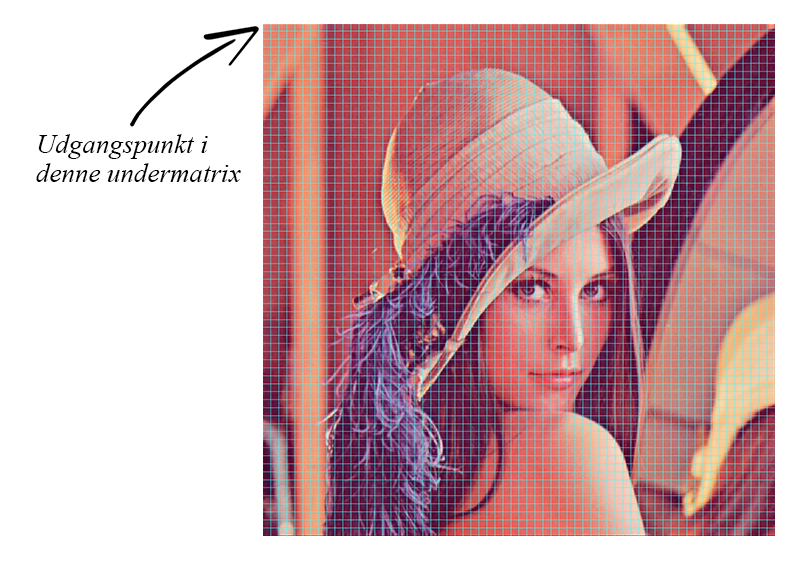
\includegraphics[width=0.7\textwidth]{billeder/lena-grid.png}
\caption{Lena delt op i 4096, $8 \times 8$ undermatricer.}
\label{fig:lena-grid-8x8}
\end{figure}

Herfra udføres DCT på undermatricen, og B findes vha. $B = U \boldsymbol{\cdot} A \boldsymbol{\cdot} U^T$, hvor $U$ og $U^T$ er givet i udtryk \vref{eq:DCTmatrix}.

\begin{figure}[!h]
\begin{minipage}[b]{0.25\linewidth}
\centering

\includegraphics[width=\textwidth]{Billeder/LenaAnvendelse/RED8x8/lena2-R8x8-DCT.png}
\caption{DCT - Visuel.}
\label{fig:lena2-R8x8-DCT-visuel}
\end{minipage}
\hspace{0.5cm}
\begin{minipage}[b]{0.40\linewidth}
\centering
\[B_{1,\ 1}=\begin{bmatrix}
791    & -71  & 8,12   & 4,23   & -1,8  & -3,6  & -1,2  & 2,49   \\
-1,5  & 0,43  & 0,01   & 1,90   & 0,78  & 1,25   & -3,4  & -0,9 \\
-0,7 & -0,8 & -0,7 & -0,9 & -0,1 & -0,2 & 0,93  & 1,02   \\
2,66   & 1,02   & 1,38   & 0,21  & -0,5 & -0,5 & 0,95  & -1,3  \\
-3,3  & -0,9 & -1,5  & -0,2 & 0,75  & 0,18  & -1,0  & 1,55   \\
2,40   & 0,53  & 1,12   & 0,85  & -0,6 & 0,75  & -0,4 & -1,7  \\
-1,1  & -0,1 & -0,6 & -1,3  & 0,32  & -1,4  & 1,75   & 1,50   \\
0,21  & -0,1 & 0,18  & 0,98  & -0,1 & 1,15   & -1,6  & -0,9 \\
\end{bmatrix}\]
\caption{DCT - Tal.}
\label{fig:lena2-R8x8-DCT-matrix}
\end{minipage}
\end{figure}

Det ses tydeligt på den visuelle figur \ref{fig:lena2-R8x8-DCT-visuel}, hvordan alle overflødige høje frekvenser allerede er reduceret kraftigt. Dette er nøjagtigt det, som ønskes af DCT'en, da de lave frekvenser kan ses tydeligere af øjet end de høje. Den visuelle repræsentation er fremkommet ved at trunkere dataene til intervallet $[0;255]$. Næste trin i algoritmen er kvantiseringen, hvor der i dette eksempel tages udgangspunkt i $Q50$ jævnfør \vref{eq:Q50teori}. Den afrundede $C$ findes vha. $\lfloor C_{(i,\ j)} \rceil = \frac{B_{(i,\ j)}}{Q50_{(i,\ j)}}$:

\begin{figure}[!h]
\begin{minipage}[b]{0.25\linewidth}
\centering

\includegraphics[width=\textwidth]{Billeder/LenaAnvendelse/RED8x8/lena3-R8x8-quantization.png}
\caption{Kvantisering - Visuel.}
\label{fig:lena3-R8x8-quantization-visuel}
\end{minipage}
\hspace{0.5cm}
\begin{minipage}[b]{0.40\linewidth}
\centering
\[C_{1,\ 1}=\begin{bmatrix}
49 & -1 & 1 & . & . & . & . & . \\
.  & .  & . & . & . & . & . & . \\
.  & .  & . & . & . & . & . & . \\
.  & .  & . & . & . & . & . & . \\
.  & .  & . & . & . & . & . & . \\
.  & .  & . & . & . & . & . & . \\
.  & .  & . & . & . & . & . & . \\
.  & .  & . & . & . & . & . & . \\
\end{bmatrix}\]
\caption{Kvantisering - Tal.}
\label{fig:lena3-R8x8-quantization-matrix}
\end{minipage}
\end{figure}

Bemærk at der bruges indgangsvis division. Det ses, jævnfør tallene på figur \ref{fig:lena3-R8x8-quantization-matrix}, at matricen hovedsageligt udgøres af nuller. Dette er essentielt for Huffmankodningen, da den nu effektivt kan komprimere. Huffman-træet for undermatricen kan ses på figur \ref{fig:Huffman-8x8-visuel}. Tallene uden parentes repræsenterer hyppigheden af tallene i parentes.
\begin{figure}[htbp]
\centering
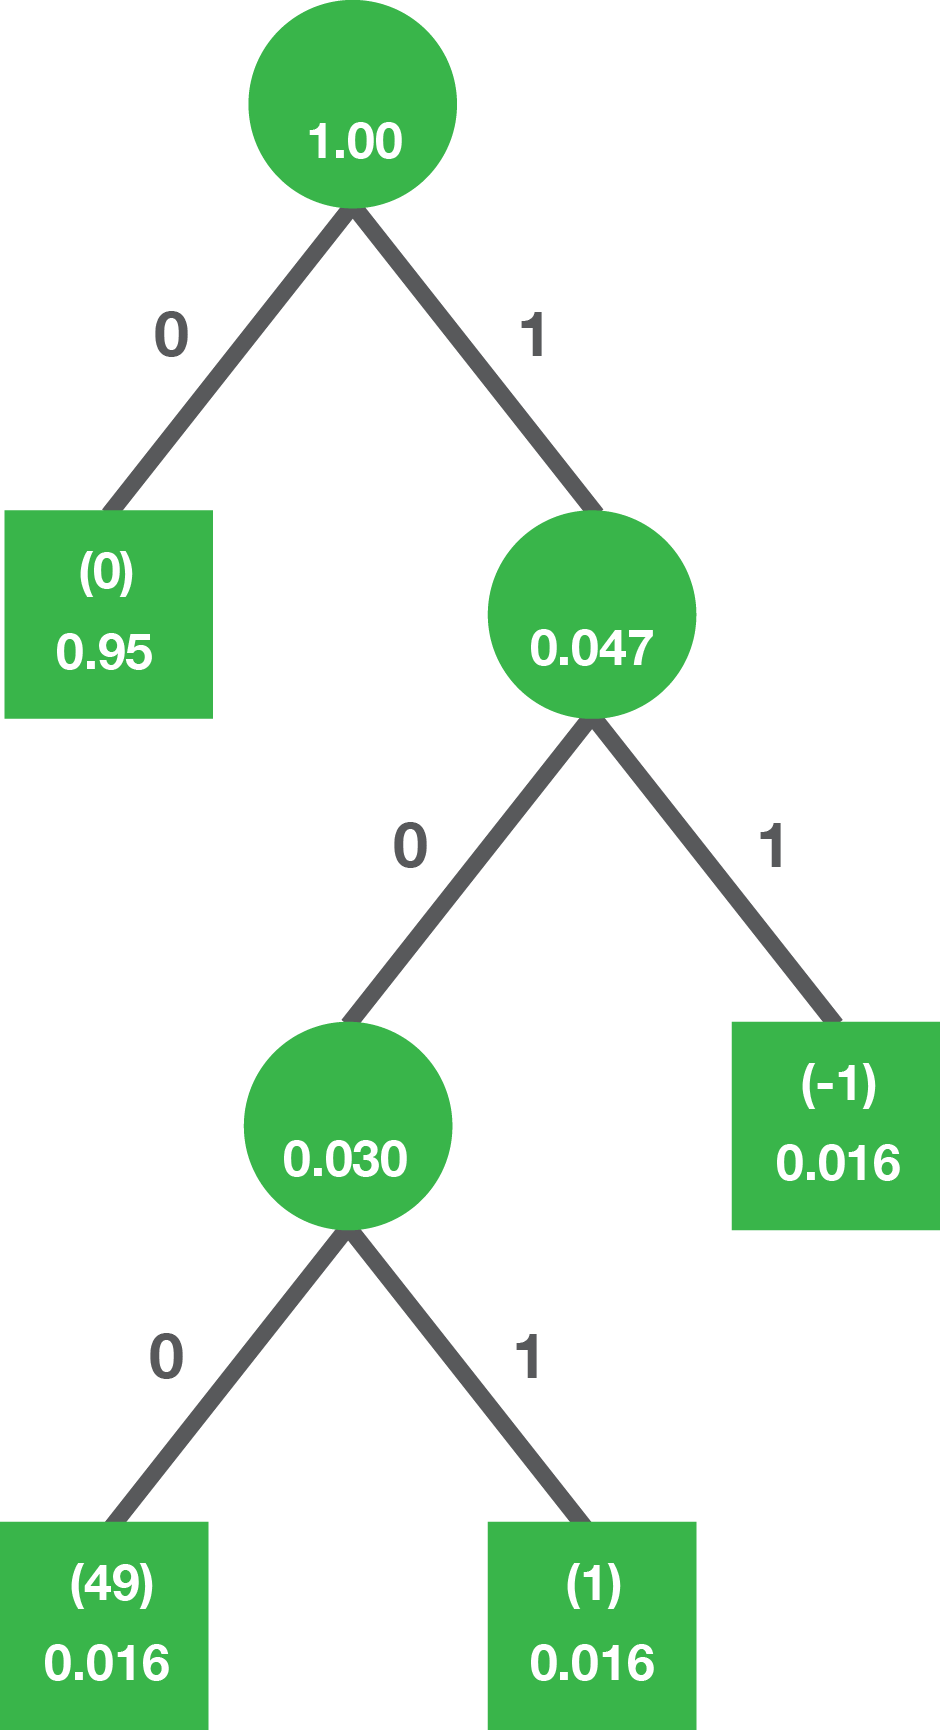
\includegraphics[width=0.25\textwidth]{Billeder/LenaAnvendelse/HUFFMAN/Huffman-8x8.png}
\caption{Huffman-træ for undermatricen.}
\label{fig:Huffman-8x8-visuel}
\end{figure}

Træet havde mildt sagt været markant større, hvis at Huffmantræet var lavet ud fra eksempelvis  $A_{1,\ 1}$ eller $B_{1,\ 1}$. Her er det åbenlyst hvordan de to nævnte matricer, kun er \textit{forberedende} for en effektiv komprimering.

Der kan med fordel opstille en tabel med relevante observationer fra Huffmantræet og dens resultater, se tabel \ref{tb:Huffman-8x8}. Den binære form blev fundet jævnfør \vref{sec:huffmanteori}.

\begin{table}[!h]
\centering
\begin{tabular}{|l|l|l|l|}
\hline
\textbf{Indgangsværdi} & \textbf{Antal} & \textbf{Sandsynlighed}      & \textbf{Binær form} \\ \hline
49                & 1              & $\frac{1}{64} \approx 0,016$ & 100                 \\ \hline
1                 & 1              & $\frac{1}{64} \approx 0,016$ & 101                 \\ \hline
-1                & 1              & $\frac{1}{64} \approx 0,016$ & 11                  \\ \hline
0                 & 61             & $\frac{61}{64} \approx 0,95$ & 0                   \\ \hline
\end{tabular}
\caption{Huffman-træet i tabelform}
\label{tb:Huffman-8x8}
\end{table}

I binær form vil undermatricen nu hedde: $$ 100110001010000000000000000000000000000000000000000000000000000000000 $$
En komprimeret fil er opnået, og den lange streng af nuller resulterer i, at filen fylder mindre, end hvis Huffmankodningen var blevet gjort før kvantiseringen. Jævnfør algoritmen på side \pageref{tb:Algoritme-Dekomprimering-DCT} udføres \textit{de}komprimeringen, hvilket gøres med de modsatte regneoperationer i forhold til komprimeringen.

\begin{table}[!h]
\centering
\begin{tabular}{lll}
\hline
\multicolumn{2}{l}{\textbf{Algoritme: Dekomprimering vha. DCT}}    &                                                                   \\ \hline
\\
\multicolumn{1}{|l}{1.}        & Input:                     & Komprimeret fil \\
\multicolumn{1}{|l}{2.}        & Output:                    & Dekomprimeret billede, $A'$                                           \\
                               &                            &                                                                   \\
\multicolumn{2}{|l}{\textit{Dekomprimering (invers proces)}} &                                                                   \\
\multicolumn{1}{|l}{9.}        & Entropi dekodning:         & Filen dekomprimeres vha. Huffman til $C'$             \\
\multicolumn{1}{|l}{10.}        & Dekvantisering:            & $B' = Q_{(i,\ j)} \cdot C'_{(i,\ j)}$                                                 \\
\multicolumn{1}{|l}{11.}       & Invers DCT / DCT-III:      & $A' = U^T \boldsymbol{\cdot} B' \boldsymbol{\cdot} U$\\
\multicolumn{1}{|l}{12.}       & Decentrering omkring 0:      & $A' = A' + 128$ indgangsvist\\
\multicolumn{1}{|l}{13.}       & Samling:                   & $8 \times 8$ matricer samles til ét billede
\\  
\end{tabular}
\label{tb:Algoritme-Dekomprimering-DCT}
\end{table}

Resultatet af den inverse algoritme på $A_{(1,\ 1)}$ ender med følgende værdierne som illustreret i figur \ref{fig:lena4-R8x8-compressed-visuel} og \ref{fig:lena4-R8x8-decompressed-matrix}.

\begin{figure}[htbp]
\begin{minipage}[b]{0.27\linewidth}
\centering

\includegraphics[width=\textwidth]{Billeder/LenaAnvendelse/RED8x8/lena4-R8x8-compressed.png}
\caption{Dekomprimeret - Visuel.}
\label{fig:lena4-R8x8-compressed-visuel}
\end{minipage}
\hspace{0.5cm}
\begin{minipage}[b]{0.45\linewidth}
\centering
\[C_{1,\ 1}=\begin{bmatrix}
226 & 225 & 224 & 224 & 225 & 226 & 228 & 230 \\
226 & 225 & 224 & 224 & 225 & 226 & 228 & 230 \\
226 & 225 & 224 & 224 & 225 & 226 & 228 & 230 \\
226 & 225 & 224 & 224 & 225 & 226 & 228 & 230 \\
226 & 225 & 224 & 224 & 225 & 226 & 228 & 230 \\
226 & 225 & 224 & 224 & 225 & 226 & 228 & 230 \\
226 & 225 & 224 & 224 & 225 & 226 & 228 & 230 \\
226 & 225 & 224 & 224 & 225 & 226 & 228 & 230 \\
\end{bmatrix}\]
\caption{Dekomprimeret - Tal.}
\label{fig:lena4-R8x8-decompressed-matrix}
\end{minipage}
\end{figure}

Den umiddelbare største ændring af undermatricen er dens endnu mere ensartethed. Da der ikke forekommer drastiske spring i overgangene mellem pixelene ser den monoton ud. Det er svært for det menneskelige øje, at skældne mellem denne undermatrice og den oprindelige, hvilket var intentionen i første omgang. 
For referencens skyld udføres algoritmen på hele Lena-billedet i de følgende figurer. Det undlades dog at vise den binære form.

%\begin{figure}[!h]
%\begin{minipage}{0.45\textwidth}
%\centering
%
\includegraphics[width=0.4\textwidth]{Billeder/LenaAnvendelse/LENABILLEDE/lena2-DCT.png}
%\caption{DCT - Lena.}
%\label{fig:lena2-DCT-visuel}
%\end{minipage}
%\hspace{0.5cm}
%\begin{minipage}{0.45\textwidth}
%\centering
%
\includegraphics[width=0.4\textwidth]{Billeder/LenaAnvendelse/LENABILLEDE/lena4-enhanced-quantization2.png}
%\caption{Kvantisering - Lena.}
%\label{fig:lena4-enhanced-quantization-visuel}
%\end{minipage}
%\end{figure}
\begin{figure}[htbp]
\begin{minipage}{0.3\textwidth}
\centering
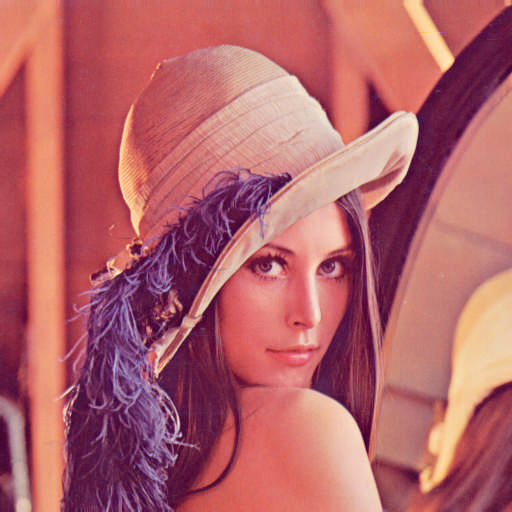
\includegraphics[width=0.9\textwidth]{Billeder/LenaAnvendelse/LENABILLEDE/lena5-compressed.png}
\caption{\href{https://www.dropbox.com/home/P1\%20-\%20B205/vejleder/billeder/DCT/Lena\%20ved\%20forskelige\%20Q?preview=lenaQ50.png}{Dekomprimeret - Lena.}}
\label{fig:lena5-decompressed-visuel}
\end{minipage}
\hspace{0.5cm}
\begin{minipage}{0.3\textwidth}
\centering

\includegraphics[width=0.9\textwidth]{Billeder/fejlbilleder/fejl50.png}
\caption{\href{https://www.dropbox.com/home/P1\%20-\%20B205/vejleder/billeder/DCT/Fejlbilleder?preview=fejl50.png}{Fejlbillede - Lena.}}
\label{fig:lena1-org-fejl}
\end{minipage}
\hspace{0.5cm}
\begin{minipage}{0.3\textwidth}
\centering
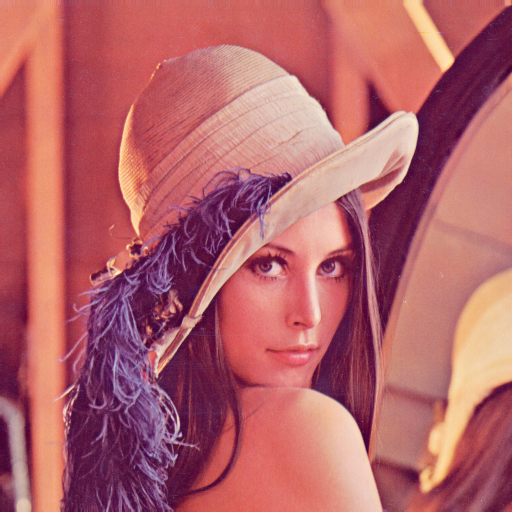
\includegraphics[width=0.9\textwidth]{Billeder/LenaAnvendelse/LENABILLEDE/lena1-org.png}
\caption{\href{https://www.dropbox.com/home/P1\%20-\%20B205/vejleder/billeder?preview=lena-org.tiff}{Oprindelig - Lena.}}
\label{fig:lena1-org-visuel}
\end{minipage}
\end{figure}

Jævnfør \ref{fig:lena5-decompressed-visuel} og \ref{fig:lena1-org-visuel} er det enormt svært at skelne mellem billederne. Dette forstærkes ydermere af fejlbilledet, der illustrerer forskellen mellem det nye og det oprindelige billede. Grå illustrerer ingen forskel, sort illustrerer en mørkere farve i det nye billede, og ligeså illustrerer en lysere farve, at det nye billede er blevet lysere. En farvenuance illustrerer en farveforskel. Hensigten er opnået; billedet har ikke ændret sig betydeligt, og filstørrelsen er komprimeret i forhold til før algoritmen.